\documentclass[11pt]{article}
\usepackage{amsmath, amssymb}
\usepackage{geometry}
\geometry{margin=1in}
\usepackage{fancyhdr}
\usepackage{lastpage}
\usepackage{parskip} % Better paragraph spacing
\usepackage{titlesec} % Better section formatting
\usepackage{graphicx}
\usepackage{float}
\usepackage[most]{tcolorbox}
\usepackage{lmodern}
\usepackage{caption}
\usepackage{hyperref}

% Define commands for reusable content
\newcommand{\coursename}{COM-402 Advanced Networks}
\newcommand{\lecturenum}{07}
\newcommand{\lecturedate}{\today}
\newcommand{\professor}{Pavlos Nikoupoulos}

\hypersetup{colorlinks=true,linkcolor=blue,urlcolor=blue}

% Configure section spacing
\titlespacing*{\section}{0pt}{2ex plus 1ex minus .2ex}{1.5ex plus .2ex}
% Header / Footer
\pagestyle{fancy}
\fancyhf{}
\fancyhead[L]{\coursename}
\fancyhead[R]{Lecture \lecturenum}
\fancyfoot[L]{EPFL - Computer Science}
\fancyfoot[C]{Author: Jonathan Dutoit}
\fancyfoot[R]{Page \thepage\ of \pageref{LastPage}}

\begin{document}

\begin{center}
  {\large EPFL - Computer Science} \\[0.5em]
  {\Large \textbf{\coursename}} \\[0.5em]
  {\large Lecture \lecturenum\ --- \lecturedate} \\[0.5em]
  {\large Author: Jonathan Dutoit} \\[0.5em]
  {\large Professor: \professor} \\[0.5em]
\end{center}

\vspace{1cm}

\begin{center}
  {\LARGE \textbf{Transporter Layer Continued}}
\end{center}

% Quick centered image
\begin{figure}[H]
    \centering
    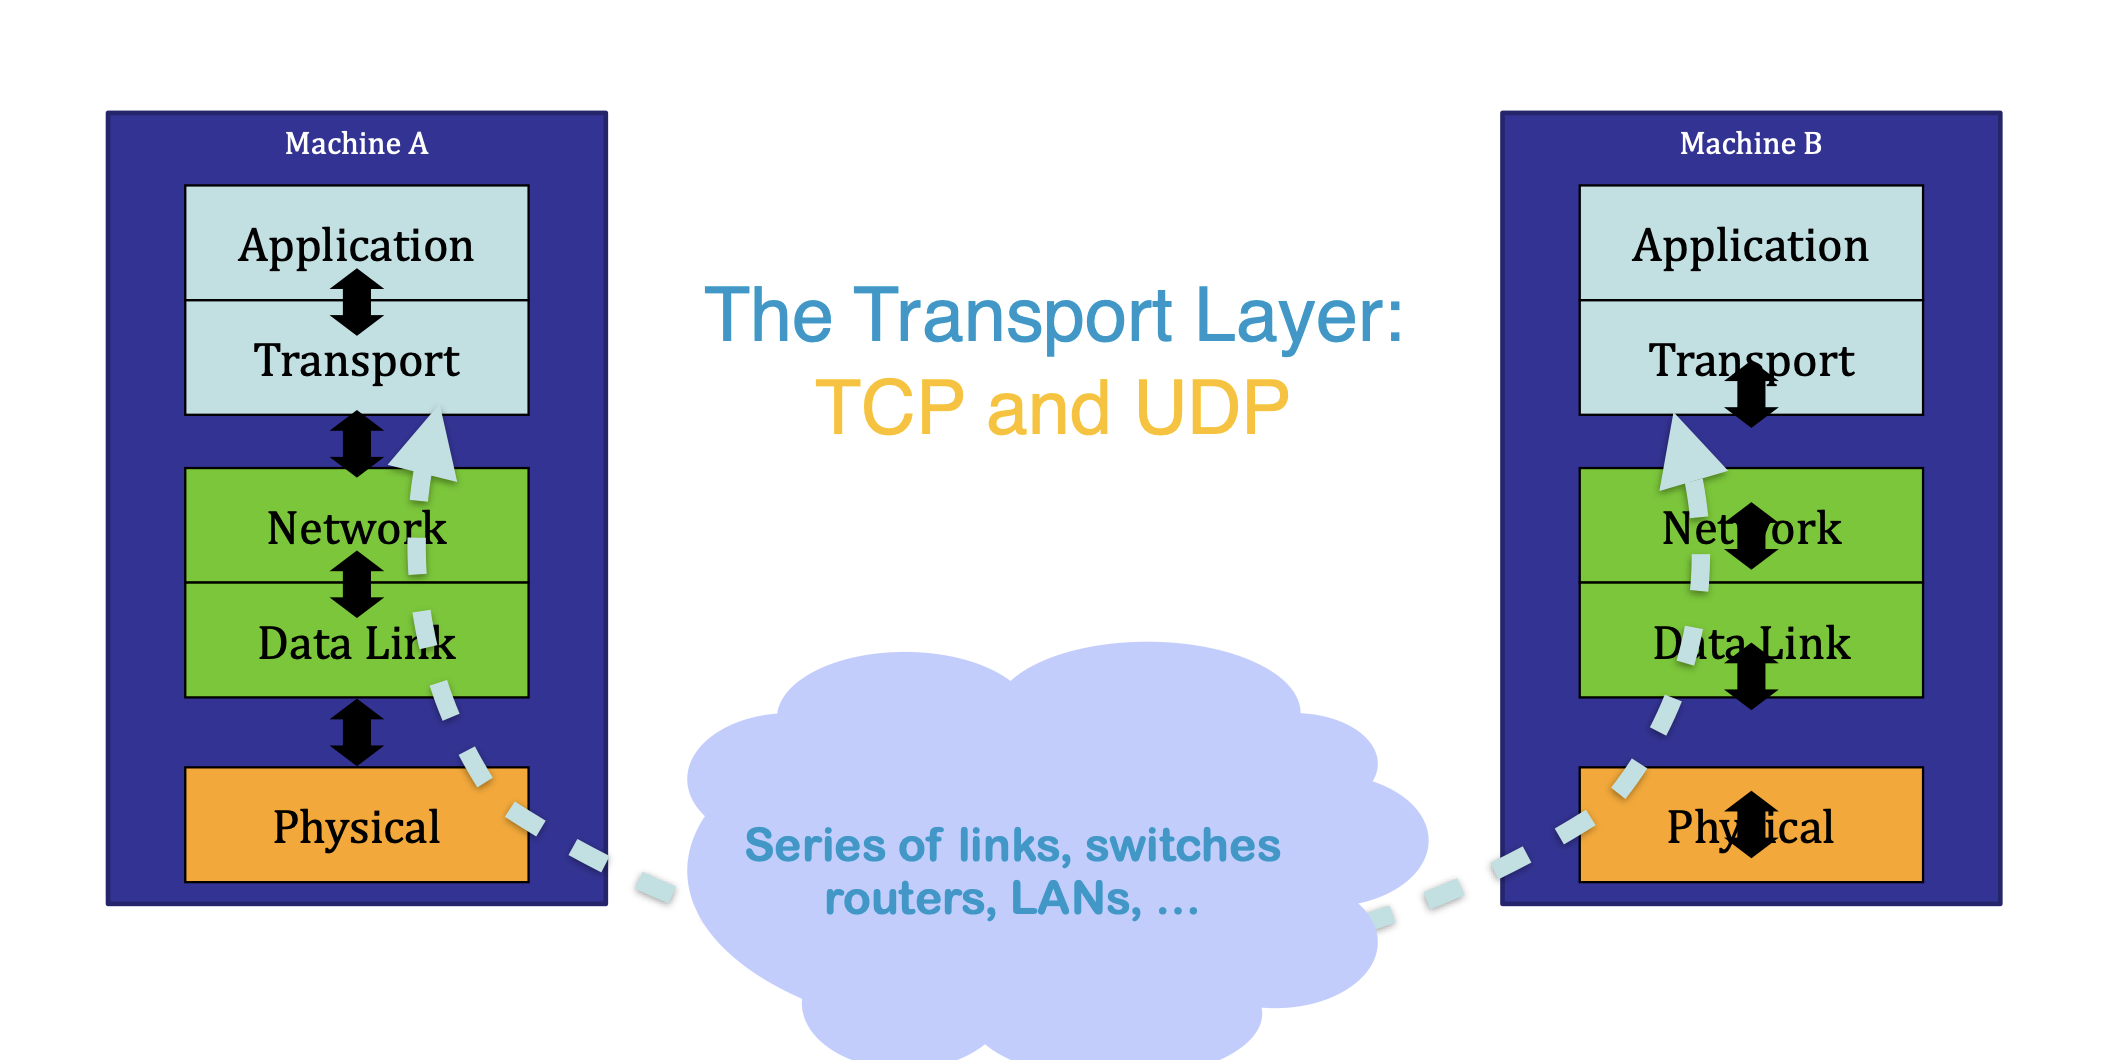
\includegraphics[width=0.65\textwidth]{transport-layer}
    \label{fig:LABEL}
\end{figure}
\vspace{1cm}

\begin{tcolorbox}[
  colback=gray!15,     % background color
  colframe=black!50,    % border color
  boxrule=1pt,       % border thickness
  arc=3mm,             % rounded corners
  left=4mm, right=4mm, top=2mm, bottom=2mm % padding
]
\textbf{Window size = 4'000 bytes, one packet = 1'000 bytes. At time $t_0$, the usable part of the sliding window is 4000, and there is a lot of data in the socket to be sent. So, the sender sends 4 segments. At time  $t_1$, sender...}

% Quick centered image
\begin{figure}[H]
    \centering
    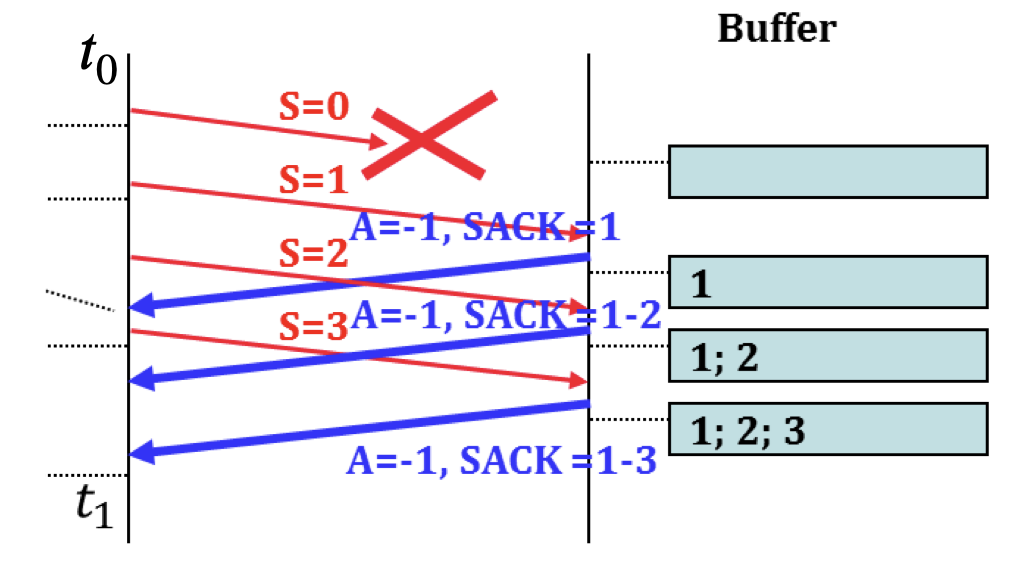
\includegraphics[width=0.4\textwidth]{sliding-window-question}
    \label{fig:LABEL}
\end{figure}
\vspace{0.2cm}

A. Can send segment S=4\\
B. Cannot send segment S=4 \\
C. It depends on whether data was consumed by application \\
D. I do not know \\

\textbf{Answer:} B. \\ 
Packet 4 it outside the window [0:3] and cannot be sent. It has to wait until the loss of packet 0 is repaired, which happens at time $t_2$
\end{tcolorbox}

\begin{itemize}
	\item Sender needs a \textcolor{blue}{\textit{retransmission buffer}} to hold unack'ed data; its size is equal to the window size. 
	\item Segments are removed from the resequencing/receive buffer when they are finally put in order and application reads them. 
\end{itemize}

\subsection*{A fixed-size (static) window cannot prevent receive-buffer \textcolor{red}{\textit{overflows}}}


\section*{TCP Sockets (simplified scenario)}

\section*{Why both TCP and UDP?}

Most applications nowadays use TCP, as this avoids re-inventing error recovery for each app. But some apps may not need TCP-like error recovery (i.e., packet retransmission): 
\begin{itemize}
	\item Voice applications / Sensor data streaming \\
	\textcolor{blue}{}
	\item An application that sends just one message, like name resolution (DNS)
	\item Multicast (TCP does not support multicast IP addresses)
\end{itemize}

\section*{4. More TCP Bells and Whistles}

How to deal with \textbf{corner cases}? Suppose that an application writes few bytes in socket; should TCP create a segment or wait for more bytes? 
\begin{itemize}
	\item \textcolor{blue}{Nagle's algorithm}: send \verb|min{bytes written in one RTT, MSS}|
\end{itemize}

How to handle silly window-increase advertisements by 1 byte? The idea is similar to Nagle's, we do something simple

Window field is 16 bits $\Rightarrow$ ma throughput even for RTT=1msec is $\tilde$ 524Mbps; can we do better?

\begin{itemize}
	\item negotiate a \textcolor{blue}{scaling factor} of the window during connection setup (RFC1323)
\end{itemize}

\section*{How to detect packet loss?}

Packet loss in TCP is detect via \textcolor{red}{times} and \textcolor{red}{duplicates} ACKs.

The main timers are called \textcolor{blue}{retransmission timeouts (RTO)}, it's set for every packet transmission and when a timer expires (= \textcolor{red}{timeout}), this is interpreted as \textcolor{red}{severe loss} in the channel. Thus, all timers are reset and all un-acknowledged data is marked as needing retransmission

A \textcolor{blue}{duplicate ACK} = a TCP segment where the cumulative ACK value repeats a previously received ACK value. This is interpreted as \textcolor{red}{not-so-severe loss} in the channel. 

\textcolor{blue}{Timers use an estimate of round trip time (RTT)}

\textcolor{red}{Why?} RTO timer must be set to a value $\geq$ RTT, but not too much

 \textcolor{red}{What?} RTT estimation gives an upper bound on the round trip time, used to set the RTO

 \textcolor{red}{How?}
\end{document}	
